%
% PSI Programmer's Manual
%
% CVS Revision Control Section
%
% TDC, February, 1996
% Modified by TDC, December 2002
%

The concurrent versions system (CVS) (\htmladdnormallink{{\tt
www.cvshome.org}}{http://www.cvshome.org}) provides a convenient means by
which programmers may obtain the latest (or any previous) version of the
\PSIthree\ source from the main repository or a branch version, add new
code to the source tree or modify existing \PSIthree\ modules, and then
make changes and additions available to other programmers by checking the
modifications back into the main repository.  CVS also provides a ``safety
net'' in that any erroneous modifications to the code may be easily removed
once they have been identified.  This section describes how to use CVS to
access and modify the \PSIthree\ source code.  (Note that compilation and
installation instructions are given in a separate document.)

\subsection{Secure Access to the \PSIthree\ Repository} The main repository
for the \PSIthree\ Source code is currently maintained by the Crawford group
at Virginia Tech.  To check out the code, one must first obtain a CVS account
by emailing \htmladdnormallink{{\tt crawdad@vt.edu}}{mailto:crawdad@vt.edu}.
After you have a login-id and password, set the {\tt CVSROOT} environmental
variable for your shell to point to the main repository:

\noindent
For csh/tcsh:
\begin{verbatim}
setenv CVSROOT :pserver:login@sirius.chem.vt.edu:/home/users/psi3/master
\end{verbatim}

\noindent
For sh/bash:
\begin{verbatim}
CVSROOT=:pserver:login@sirius.chem.vt.edu:/home/users/psi3/master
export CVSROOT
\end{verbatim}

\noindent where {\tt login} is your login name.  Next, provide a password
to the CVS server by typing {\tt cvs login}.  (Subsequent requests to the
repository will not require you to re-login.)

\subsection{\PSIthree\ CVS Policies: Which Branch Should I Use?}
\label{section:branches}

The \PSIthree\ repository is comprised of a main trunk and several
release branches.  Which you should use depends on the development
work you plan for the codes:
\begin{enumerate}
\item The main trunk is reserved for development of new functionality.
\item Bug fixes, defined as anything that doesn't add functionality
(including documentation updates) should be made {\em only} on the most
recent stable release branch.
\end{enumerate}

\noindent Fig.~\ref{Fig:cvs} provides a schematic of the CVS revision-control
structure and branch labelling.  Two release branches are shown, the current
stable branch, named {\tt psi-3-2}, and a planned future release, to be
named {\tt psi-3-3}.  The tags on the branches indicate release points,
where bugs have been fixed and the code has been or will be exported for
public distribution.  As soon as a release branch is created, a tag will
be generated so that updates may be made to that version of the code.
We have adopted the convention that the first tag on a new release branch
will be given the suffix, {\tt -rc-1}, for ``release candidate 1'' (i.e.,
a numbered beta release).  Subsequent tags for new released on the same
branch will be updated with {\tt -rc-2}, {\tt -rc-3}, etc.  Once the
code is appropriately stable to be beyond beta status, release tags will
be given the suffic, {\tt -0}, {\tt -1}, etc., indicating patch levels.
The dotted lines in the figure indicate merge points: before each public
release, changes made to the code on the stable release branch will be
merged into the main trunk (and {\em vice versa}).

\begin{figure}[h]
\begin{center}
\epsfig{file=cvs.ps,height=3.5cm}
\end{center}
\caption{\PSIthree\ CVS branch structure with examples of branch- and
release-tag labelling.}
\label{Fig:cvs}
\end{figure}

\noindent
The following are some of the most commonly used CVS commands for checking
out and updating working copies of the \PSIthree\ source code are.

\noindent
$\bullet$ To checkout a working copy of the head of the main trunk:

{\tt cvs co psi3} 

\noindent
$\bullet$ To check out a working copy of the head of a specific release branch,
e.g., the branch labelled {\tt psi-3-2}:

{\tt cvs co -r psi-3-2}

\noindent Note that this sets a ``sticky'' branch tag, i.e. subsequent
{\tt cvs update} commands will provide updates only on the chosen branch.
Note also that after you have checked out a fresh working copy of the code
you must run the {\tt autoconf} command to generate a {\tt configure} script
for building the code.  (See the installation manual for configuration,
compilation, and testing instructions.)

\noindent
$\bullet$ To update your current working copy to include the latest revisions:

{\tt cvs update -dP}

\noindent
Notes: (a) This command should be run in the top-level of your working-copy's
source tree; (b) This will update only the revisions on your current branch;
(c) the {\tt -d} flag tells CVS to grab any new directories that have
appeared in the repository on this branch; (c) the {\tt -P} option tells
CVS to remove (prune) any empty directories from your working copy.

\noindent
$\bullet$ To convert your working copy to the head of a specific branch:

{\tt cvs update -r psi-3-2 psi3}

\noindent
$\bullet$ To convert your working copy to the head of the main trunk:

{\tt cvs update -A}

\noindent
{\bf Warning:} The previous two {\tt update} commands should be used {\sc
with caution}.  If you have made changes to your working copy but have
not yet checked them into the repository, the update to another branch
will often (always?) delete your changes!

\noindent
$\bullet$ To find out what branch your working copy is on, run this in your
top-level \PSIthree\ source directory:

{\tt cvs status -v configure.in}

\noindent
This will list all tags and branch tags available for the file (which
should a correct list for the whole \PSIthree\ repository) and it will
indicate whether your working copy is on a particular branch or not.

\noindent
The working copy of your code will be placed in the directory \file{psi3},
regardless of your choice of branch.  In this manual, we will refer to
this directory from now on as {\tt \$PSI3}.  


\noindent
Some words of advice:
\begin{enumerate}
\item Be careful!  If you aren't sure if you should run the CVS command
you're about to try, perhaps you should first make a backup of of your
working copy of the code.
\item Read the CVS manual.  Seriously.
\begin{center}
\htmladdnormallink{{\tt
http://www.loria.fr/\~{}molli/cvs/doc/cvs\_toc.html}}{http://www.loria.fr/~molli/cvs/doc/cvs\_toc.html}
\end{center}
\item If you're about to start some significant development or bug-fixes,
first update your working copy to the latest version on your branch.
In addition, if you do development over a long period of time (say weeks to
months) on a specific module or modules, be sure to run a {\tt cvs update}
occasionally. In can be {\em very} frustrating to try to check in lots
of changes, only to find out that the \PSIthree\ has changed dramatically
since your last update.
\end{enumerate}

\subsection{Checking in altered \PSIthree\ binaries or libraries}

If you have changes to Psi binaries or libraries which already exist, one
of two series of steps is necessary to check these changes in to the main
repository. The first series may be followed if all changes have been made
only to files which already exist in the current version. The second series
should be followed if new files must be added to the code in the repository.

\begin{itemize}
\item No new files need to be added to the repository. We will use
\library{libciomr} as an example. 
\begin{enumerate}
\item {\tt cd \$PSI3/src/lib/libciomr}
\item {\tt cvs ci}
\item Edit the comment file that CVS provides. 
\end{enumerate}
\item New files must be added to the repository. Again, we use 
\library{libciomr}
as an example. Suppose the new file is named \file{great\_code.c} .
\begin{enumerate}
\item {\tt cd \$PSI3/src/lib/libciomr} 
\item {\tt cvs add great\_code.c} 
\item {\tt cvs ci}
\item Edit the comment file that CVS provides.
\end{enumerate}
\end{itemize}

The \file{cvs ci} command in both of these sequences will examine all of
the code in the current \file{libciomr} directory against the current
version of the code in the main repository. Any files which have been
altered (and for which no conflicts with newer versions exist!) will be
identified and checked in to the main repository (as well as the new file
in the second situation).  CVS will open a comment file for editing; you
should enter a description of the changes you have made to the code here,
as well as in the code itself.  Exit the editing of the comment file,
and CVS will check the new code into the main repository.

\subsection{Adding entirely new code to the main \PSIthree\ repository} 
\label{checkin_new}

If the programmer is adding a new executable module or library to the
\PSIthree\ repository, a number of important conventions should be followed:

\begin{enumerate}
\item Since such changes almost always involve additional functionality,
new modules or libraries should be added only on the main CVS trunk.
See section \ref{section:branches} for additional information.

\item The directory containing the new code should be given a name
which matches the name of the installed code (e.g. if the code
will be installed as \module{newcode}, the directory containing
the code should be named \file{newcode}). New executable modules
must be placed in \shellvar{\$PSI3}\file{/src/bin} and libraries in
\shellvar{\$PSI3}\file{/src/lib} of the user's working copy.

\item The Makefile should be converted to an input file for the configure
script (\file{Makefile.in} --- see any of the current \PSIthree\ binaries
for an example) and should follow the conventions set up in all of the
current \PSIthree\ \file{Makefiles}. This includes use of \file{MakeVars}
and \file{MakeRules}.

\item New binaries should be added to the list contained in
\shellvar{\$PSI3}\file{/src/bin/Makefile.in} so that they will be compiled
automatically when a full compilation of the \PSIthree\ distribution
occurs. This step is included in the sequence below.

\item A documentation page should be included with the new code (see
section \ref{Documentation} for more information). As a general rule,
if the code is not ready to have a documentation page, it is not ready
to be installed in \PSIthree. 

\item The \file{configure.in} file must be altered so that users may check
out copies of the new code and so that the \file{configure} script will
know to create the Makefile for the new code. These steps are included in
the sequence below.

\end{enumerate}

Assume the new code is an executable module and is named
\module{great\_code}. The directory containing the new code must contain
only those files which are to be checked in to the repository! Then the
following steps will check in a new piece of code to the main repository:

\begin{enumerate}
\item {\tt cd \$PSI3/src/bin}
\item {\tt cvs add great\_code}
\item Answer ``y'' when CVS asks if you wish to create the new directory in
      the repository. 
\item {\tt cd great\_code}
\item {\tt cvs add *}
\item {\tt cvs ci}
\item Edit the comments file that CVS provides. 
\item {\tt cd \$PSI3}
\item Edit \file{configure.in} and add \file{great\_code} to the list. 
\item {\tt cvs ci}
\item Edit the comments file that CVS provides. 
\item {\tt autoconf} 
\item {\tt cd \$PSI3/src/bin} 
\item Edit \file{Makefile.in} and add \file{great\_code} to the list. 
\item {\tt cvs ci}
\item Edit the comments file that CVS provides. 
\end{enumerate}
At this point, all of the code has been properly checked in. However, you must
test to make sure that the code can be checked out by other programmers, and
that it will compile correctly. The following steps 
will store your personal version of the code, check out the new code, and
test-compile it:
\begin{enumerate}
\item {\tt cd \$PSI3/src/bin}
\item {\tt mv great\_code great\_code.bak}
\item {\tt cd \$PSI3/..}
\item {\tt cvs co \$PSI3/src/bin/great\_code}
\item {\tt cd \$objdir}
\item {\tt \$PSI3/configure -}{\tt -prefix=\$prefix}
\item {\tt cd src/bin/great\_code}
\item {\tt make install}
\end{enumerate}
(Note that \$prefix and \$objdir to the installation and compilation
 directories defined in the \PSIthree\ installation instructions.)
Your original version of the code remains under \file{great\_code.bak},
but should be no longer necessary if the above steps work. Note that it is
necessary to re-run \file{configure} explicitly, instead of just running
\file{config.status}, because the latter contains no information about
the new code.

\subsection{Updating checked out code}

If the code in the main repository has been altered, other users' working
copies will of course not automatically be updated.  In general, it is
only necessary to execute the following steps in order to completely update
your working copy of the code:

\begin{enumerate}
\item {\tt cd \$PSI3}
\item {\tt cvs update -dP}
\end{enumerate}

This will examine each entry in your working copy and compare it to the most
recent version in the main repository. When the file in the main repository
is more recent, your version of the code will be updated. If you have made
changes to your version, but the version in the main repository has not
changed, the altered code will be identified to you with an ``M''. If you
have made changes to your version of the code, and one or more newer versions
have been updated in the main repository, CVS will examine the two versions
and attempt to merge them -- this process usually has conflicts however,
and is sometimes unsuccessful. You will be notified of any conflicts that
arise (labelled with a ``C'') and you must resolve them manually.

The {\tt -dP} flags to {\tt cvs} above will also ensure that any
directories added to or removed from the main repository are also added or
deleted in your working copy.  Keep in mind, however, that the appearance
of new directories will require you to re-run the configure script to
compile the new codes.  For example,

\begin{enumerate}
\item {\tt cd \$PSI3}
\item {\tt cvs update -dP}
\item {\tt autoconf}
\item {\tt cd \$objdir}
\item {\tt \$PSI3/configure -}{\tt -prefix=\$prefix}
\item {\tt cd src/bin/great\_code}
\item {\tt make install}
\end{enumerate}
This will check out any new code that has been added to the repository since 
the last time the \file{cvs update} command was issued, correctly update 
the \file{configure} script (assuming the programmer who added the code 
followed the steps from section \ref{checkin_new} and edited the 
\file{configure.in} file), re-configure for the new code (note that
you must run \file{configure} and not \file{config.status} here), and 
then compile the code.

\subsection{Removing code from the repository}
If alterations of libraries or binaries under Psi involves the deletion of 
source code files from the code, these must be explicitly removed through CVS.

The following steps will remove a source code file named \file{bad\_code.F} 
from a binary module named \module{great\_code}:
\begin{enumerate}
\item {\tt cd \$PSI3/src/bin/great\_code}
\item {\tt rm bad\_code.F}
\item {\tt cvs remove bad\_code.F}
\item {\tt cvs ci}
\item Edit the comments file that CVS provides. 
\end{enumerate}

\subsection{Checking out older versions of the code}
It is sometimes necessary to check out older versions of a piece of code.
Assume we wish to check out an old version of \PSIdetci. If this
is the case, the following steps will do this:
\begin{enumerate}
\item {\tt cd \$PSI3/src/bin/detci}
\item {\tt cvs update -D"2 months ago"}
\end{enumerate}

This will check the main repository and provide you with the code as
it stood exactly 2 months ago. CVS is quite impressive in this respect:
It will accept all sorts of input to the -D option. You could even use
\file{-D"a fortnight ago"} and CVS would get the correct version. (But it
doesn't get \file{"two fortnights ago"} right.)  You can always get the
recent version back by simply using \file{-D"now"} or \file{-A}. Note
that subsequent updates of the current code will use the same date you
give with the \file{-D} option.  (See the CVS documentation about so-called
``sticky tags''.)

\subsection{Examining the revision history}
It can be very useful to use cvs to see what recent changes have been made to 
the code.  Anytime one checks in a new version of a file, CVS opens an
editor and requests a comment describing what changes have been made.
These comments go into a log file which may be easily
accessed through CVS.  To see what changes have been made recently
to the file \file{detci.cc}, one would go into the \file{detci} source
directory and type
\begin{verbatim}
cvs log detci.cc
\end{verbatim}

Then some summary information (such as the tags applied to the code)
is printed, and finally a list will be produced of all the versions of
the code, along with the checkin comments, in reverse chronological
order.  For example,
\begin{verbatim}
sherrill@vergil(detci)% cvs log detci.cc

RCS file: /home/users/psi3/master/psi3/src/bin/detci/detci.cc,v
Working file: detci.cc
head: 1.26
branch:
locks: strict
access list:
symbolic names:
        psi-3-2-f77-delete: 1.22
        psi-3-2-branch: 1.20.0.2
        psi-3-2-release: 1.20
        crazy-russian-tag: 1.18
        gbye-file30-branch-tag: 1.16
        gbye-file30-merge: 1.16.2.2
        gbye-file30: 1.16.0.2
        release-3-1-branch: 1.10.0.2
        rel-3-0-2dir: 1.7.0.2
        PSI_3_0_0: 1.1.1.1
        CCQC_UGA: 1.1.1
keyword substitution: kv
total revisions: 30;    selected revisions: 30
description:
description:
----------------------------
revision 1.26
date: 2002/12/24 18:54:51;  author: sherrill;  state: Exp;  lines: +1 -0
Correct a mistake in input parsing so that the argument counter is
incremented *twice* for -c [num].
----------------------------
revision 1.25
date: 2002/12/23 22:39:10;  author: sherrill;  state: Exp;  lines: +2 -2
Convert -we to -e and -quiet to --quiet
...
\end{verbatim}

Checking the log files is a very useful way to see what recent changes might 
be causing new problems with the code.

\subsection{The structure of the \PSIthree\ Source Tree}
\label{psitree} 

Your working copy of the \PSIthree\ source code includes a number of
important subdirectories:

\begin{itemize}
\item \shellvar{\$PSI3}\file{/lib} -- Source files for
  OS-independent ``library'' data.  This includes the main basis set
  data file (\file{pbasis.dat}) and the \PSIthree\ program execution
  control file (\file{psi.dat}), among others.  These files are
  installed in \file{\$prefix/share}.

\item \shellvar{\$PSI3}\file{/include} -- Source files for
  OS-independent header files, including \file{physconst.h} (whose
  contents should be obvious from its name), \file{psifiles.h}, and
  \file{ccfiles.h}, among others.  These files are installed in
  \$prefix/include.

\item \shellvar{\$PSI3}\file{/src/util} -- Source code for the utility
  program \module{tocprint}.  (Note that the \module{tmpl} module is
  no longer used and will eventually disappear.)

\item \shellvar{\$PSI3}\file{/src/lib} -- Source code for the
  libraries, including \library{libpsio}, \library{libipv1},
  \library{libchkpt}, etc.  The include files from the library
  source are used directly during the compilation of PSI to 
  avoid problems associated with incomplete installations.  Some
  include files are architecture-dependent and go in an include
  subdirectory of the compilation (object) directory.

\item \shellvar{\$PSI3}\file{/src/lib} -- Source code for the
  executable modules.
\end{itemize}

After compilation and installation, the \file{\$prefix} directory
contains the executable codes and other necessary files.  {\bf NB:}
The files in this area should never be directly modified; rather, the
working copy should be modified and the \PSIthree\ \file{Makefile}
hierarchy should handle installation of any changes.  The structure of
the installation area is:

\begin{itemize}
\item \file{\$prefix/bin} -- The main executable directory.  This
  directory must be in your path in order for the driver program,
  \module{psi3}, to find the modules.

\item \file{\$prefix/lib} -- The \PSIthree\ code libraries.  (NB: The
  description of \PSIthree\ \file{Makefiles} later in this manual will
  explain how to use the libraries.)

\item \file{\$prefix/include} -- Header files.  These are not actually
  used during the compilation of PSI but are useful for inclusion by
  external programs because they are all in the same directory.

\item \file{\$prefix/share} -- OS-independent data files, including
  basis set information.  (Do not edit this file directly; any changes
  you make can be overwritten by subsequent {\tt make} commands.)

\item \file{\$prefix/doc} -- \PSIthree\ documentation, including
  installation, programmer, and user manuals.
\end{itemize}

